% LexiMind: A Multi-Task Transformer for Summarization, Topic, and Emotion Analysis
% Educational arXiv-style paper
% Author: Oliver Perrin

\documentclass[11pt,a4paper]{article}

% ---- Layout ----
\usepackage[margin=1in]{geometry}
\usepackage{microtype}

% ---- Fonts (Times-like, matching arXiv convention) ----
\usepackage{mathptmx}
\usepackage[scaled=0.92]{helvet}
\usepackage{courier}

% ---- Math ----
\usepackage{amsmath,amssymb,amsfonts}
\usepackage{bm}

% ---- Tables and figures ----
\usepackage{booktabs}
\usepackage{multirow}
\usepackage{array}
\usepackage{caption}
\usepackage{subcaption}
\usepackage{float}

% ---- TikZ ----
\usepackage{tikz}
\usetikzlibrary{shapes.geometric,arrows.meta,positioning,fit,calc,backgrounds,
    decorations.pathreplacing,patterns}

% ---- Code listings ----
\usepackage{listings}
\lstset{
    basicstyle=\ttfamily\small,
    breaklines=true,
    frame=single,
    language=Python,
    keywordstyle=\color{blue!70!black},
    commentstyle=\color{green!50!black},
    stringstyle=\color{red!60!black},
    showstringspaces=false,
    numbers=left,
    numberstyle=\tiny\color{gray},
    xleftmargin=2em
}

% ---- References ----
\usepackage[numbers]{natbib}
\usepackage{hyperref}
\hypersetup{
    colorlinks=true,
    linkcolor=blue!60!black,
    citecolor=blue!60!black,
    urlcolor=blue!60!black
}

% ---- Misc ----
\usepackage{enumitem}
\usepackage{xcolor}

% ---- Section formatting ----
\usepackage{titlesec}
\titleformat{\section}{\large\bfseries}{\thesection}{1em}{}
\titleformat{\subsection}{\normalsize\bfseries}{\thesubsection}{1em}{}

% ---- Convenience macros ----
\newcommand{\lexiname}{\textsc{LexiMind}}
\newcommand{\tflant}{FLAN-T5}
\newcommand{\rmsnorm}{\text{RMSNorm}}
\newcommand{\softmax}{\text{softmax}}
\renewcommand{\R}{\mathbb{R}}
\newcommand{\gelu}{\text{GELU}}

\title{\lexiname{}: A Multi-Task Encoder--Decoder Transformer\\
for Summarization, Topic Classification, and Emotion Detection}

\author{
  Oliver Perrin\\
  Department of Computer Science\\
  Appalachian State University\\
  \texttt{perrinot@appstate.edu, oliver.t.perrin@gmail.com}
}

\date{January 2026}

\begin{document}
\maketitle

% =====================================================================
\begin{abstract}
% =====================================================================

\noindent We present \lexiname{}, a multi-task natural language processing system built on a custom reimplementation of the Transformer encoder--decoder architecture.
Rather than treating a pre-trained model as a black box, we construct every component---attention mechanisms, feed-forward networks, normalization layers, and positional encodings---from first principles, then transfer pre-trained weights from Google's \tflant{}-base (272M parameters) through an explicit weight-mapping module.
This hybrid approach provides full architectural transparency while retaining the linguistic knowledge captured during large-scale pre-training.

The system performs three tasks simultaneously through hard parameter sharing: \textbf{(1)}~abstractive text summarization for literary and academic content, \textbf{(2)}~7-class topic classification, and \textbf{(3)}~28-label multi-label emotion detection.
We train on a combined corpus of 95,898 samples---49K summarization pairs (arXiv abstracts and Project Gutenberg literary descriptions), 43K GoEmotions samples, and 3.4K topic samples---using a single shared encoder with task-specific heads.

Two architectural interventions prove critical for balanced multi-task learning: \textbf{learned attention pooling} for the emotion classification head (replacing standard mean pooling), and \textbf{temperature-based task sampling} during training.
Together these eliminate negative transfer for emotion detection, improving sample-averaged F1 from 0.199 to 0.352 (+77\%).
The final model achieves a BERTScore F1 of 0.83 for summarization, 85.7\% accuracy for topic classification (95\% CI: [80.4\%, 91.0\%]), and a tuned macro F1 of 0.294 for emotion detection.
A controlled comparison against BERT-base~(110M parameters) shows that the encoder-only architecture outperforms on pure classification tasks, but cannot perform abstractive summarization---highlighting the cost and benefit of the encoder--decoder design.
Training completes in approximately 9~hours on a single consumer GPU (NVIDIA RTX~4070, 12\,GB).

All code, trained weights, and datasets are publicly available.\footnote{Code: \url{https://github.com/OliverPerrin/LexiMind} \enspace Model: \url{https://huggingface.co/OliverPerrin/LexiMind-Model} \enspace Dataset: \url{https://huggingface.co/datasets/OliverPerrin/LexiMind-Discovery} \enspace Demo: \url{https://huggingface.co/spaces/OliverPerrin/LexiMind}}
\end{abstract}

% =====================================================================
\section{Introduction}
\label{sec:intro}
% =====================================================================

The Transformer architecture~\citep{vaswani2017attention} has become the dominant paradigm in natural language processing.
Its core innovation---\emph{self-attention}---allows every token in a sequence to attend to every other token in parallel, replacing the sequential processing of recurrent models with a fully parallelizable computation.
Building on this foundation, encoder--decoder Transformers like T5~\citep{raffel2020exploring} cast \emph{all} NLP tasks as text-to-text problems, and \tflant{}~\citep{chung2022scaling} further enhances T5 through instruction fine-tuning on over 1,000 diverse tasks.

Despite the power of these pre-trained models, they are typically consumed as opaque APIs---download, fine-tune, deploy.
Their internal mechanics remain hidden behind framework abstractions, making it difficult to (a)~understand \emph{why} a model behaves as it does, (b)~customize individual components for new tasks, or (c)~diagnose training pathologies.

\lexiname{} takes a different approach.
We implement a complete Transformer encoder--decoder from scratch, building each module---multi-head attention, gated feed-forward networks, RMSNorm, relative position bias---as a standalone, documented component.
We then load pre-trained weights from \tflant{}-base into this custom architecture through a carefully designed factory module that maps between parameter naming conventions.
The result is a system that combines the linguistic knowledge of large-scale pre-training with the transparency and flexibility of a from-scratch implementation.

On top of this shared backbone, we attach three task-specific heads:
\begin{enumerate}[nosep]
    \item A \textbf{decoder with language modeling head} for abstractive summarization of literary and academic texts.
    \item A \textbf{classification head with learned attention pooling} for 28-label multi-label emotion detection.
    \item A \textbf{classification head with mean pooling} for 7-class topic classification.
\end{enumerate}

The key contributions of this work are:
\begin{itemize}[nosep]
    \item A complete, modular Transformer reimplementation compatible with T5-family weight loading, serving as both a practical system and an educational reference.
    \item A multi-task architecture supporting both generative (seq2seq) and discriminative (classification) tasks from a shared encoder.
    \item A demonstration that \textbf{architectural isolation of task-specific components (attention pooling) combined with balanced optimization (temperature-based task sampling) converts negative transfer to positive transfer} in heterogeneous multi-task learning---the central empirical finding of this work.
    \item A curated training corpus of 95,898 samples across literary, academic, and conversational domains.
    \item A complete training infrastructure with mixed-precision support, gradient checkpointing, \texttt{torch.compile}, and MLflow experiment tracking, designed to run on consumer GPUs.
\end{itemize}

This paper is organized as follows.
Section~\ref{sec:background} reviews the Transformer architecture and relevant prior work.
Section~\ref{sec:architecture} describes \lexiname{}'s architecture in detail, building from primitive components up to the full multi-task system.
Section~\ref{sec:weight_transfer} explains the weight transfer mechanism from \tflant{}.
Section~\ref{sec:training} covers the training pipeline and datasets.
Section~\ref{sec:results} presents experimental results, and Section~\ref{sec:discussion} discusses findings and limitations.

% =====================================================================
\section{Background and Related Work}
\label{sec:background}
% =====================================================================

\subsection{The Transformer Architecture}

The Transformer~\citep{vaswani2017attention} consists of stacked \emph{encoder} and \emph{decoder} blocks.
Each encoder block contains two sublayers: multi-head self-attention and a position-wise feed-forward network.
Each decoder block adds a third sublayer: cross-attention over encoder outputs.
Residual connections and layer normalization surround each sublayer.

\textbf{Post-LN vs.\ Pre-LN.}
The original Transformer applies Layer Normalization~\citep{ba2016layer} \emph{after} each residual connection (Post-LN).
Subsequent work~\citep{xiong2020layer} showed that applying normalization \emph{before} each sublayer (Pre-LN) significantly improves training stability, especially for deep networks.
T5 and most modern LLMs adopt Pre-LN, and so does \lexiname{}.

\textbf{RMSNorm.}
Zhang and Sennrich~\citep{zhang2019root} proposed Root Mean Square Layer Normalization (RMSNorm), which drops the mean-centering step of standard LayerNorm while retaining competitive performance.
T5 uses RMSNorm for all normalization layers, with a learned scale parameter and no bias.

\subsection{T5 and FLAN-T5}

\textbf{T5}~\citep{raffel2020exploring} introduced a unified text-to-text framework: every NLP task is converted to a sequence-to-sequence problem by prepending a task-specific prefix (e.g., ``summarize:'').
T5 introduced several architectural choices that distinguish it from the original Transformer:
\begin{itemize}[nosep]
    \item \emph{Relative position bias} instead of absolute sinusoidal embeddings---positions are encoded as a learned bias added to attention scores rather than to token embeddings.
    \item \emph{No $\sqrt{d_k}$ scaling} in attention---unlike the original Transformer, T5 omits the $1/\sqrt{d_k}$ scaling factor from attention scores.
    \item \emph{Gated feed-forward networks} with GELU~activation---three projections ($W_\text{gate}$, $W_\text{up}$, $W_\text{down}$) instead of two.
    \item \emph{Shared input/output embeddings}---the decoder's output projection shares weights with the token embedding matrix.
\end{itemize}

\textbf{\tflant{}}~\citep{chung2022scaling} enhances T5 by instruction fine-tuning on 1,836 tasks, producing substantially better zero-shot and few-shot behavior.
\lexiname{} loads pre-trained weights from \tflant{}-base (272M parameters).

\subsection{Multi-Task Learning}

Multi-task learning (MTL)~\citep{caruana1997multitask} trains a single model on multiple tasks simultaneously, encouraging shared representations and acting as an implicit regularizer.
\emph{Hard parameter sharing}---where lower layers are shared across tasks and only the final heads are task-specific---remains the dominant approach.

A known challenge in MTL is \emph{negative transfer}: when jointly training on multiple tasks degrades performance on one or more tasks compared to single-task training.
This can occur when tasks have conflicting gradient signals or when one task dominates the shared representation.
We address this through attention pooling and temperature-based task sampling (Section~\ref{sec:multitask}).

% =====================================================================
\section{Architecture}
\label{sec:architecture}
% =====================================================================

\lexiname{} implements a complete encoder--decoder Transformer from first principles, constructing the system bottom-up from five core modules: attention, feed-forward networks, normalization, positional encoding, and task-specific heads.
Figure~\ref{fig:architecture} shows the high-level system architecture.

\begin{figure}[t]
\centering
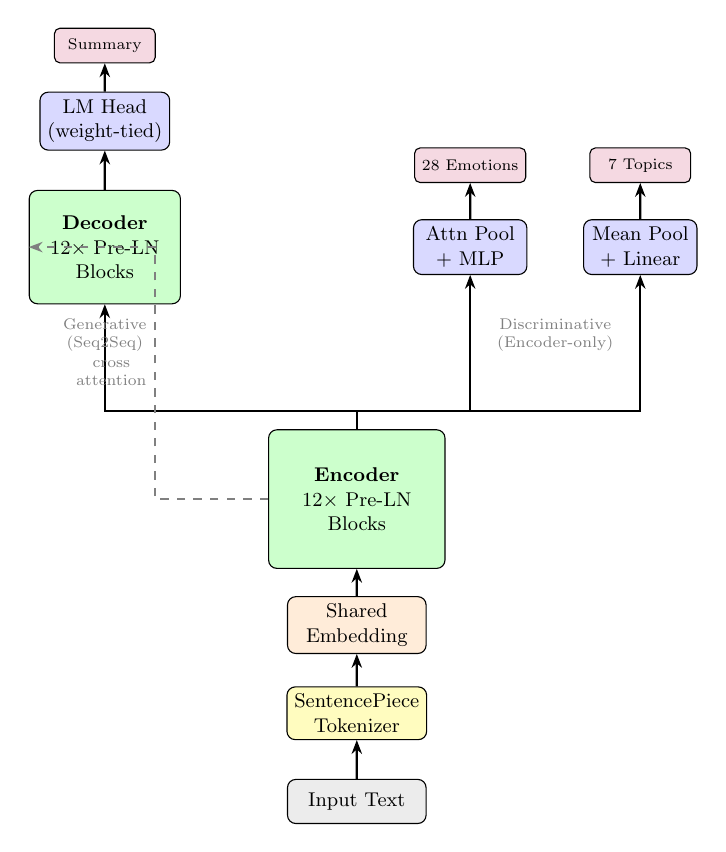
\begin{tikzpicture}[
    scale=0.8,
    transform shape,
    box/.style={draw, rectangle, minimum width=2.2cm, minimum height=0.7cm,
        align=center, rounded corners=3pt, font=\small},
    smallbox/.style={draw, rectangle, minimum width=1.6cm, minimum height=0.55cm,
        align=center, rounded corners=2pt, font=\scriptsize},
    head/.style={draw, rectangle, minimum width=1.8cm, minimum height=0.6cm,
        align=center, rounded corners=3pt, fill=blue!15, font=\small},
    arrow/.style={-{Stealth[length=5pt]}, thick},
    dashedarrow/.style={-{Stealth[length=5pt]}, thick, dashed, gray}
]

% Input
\node[box, fill=gray!15] (input) at (0, 0) {Input Text};

% Tokenizer
\node[box, fill=yellow!25] (tokenizer) at (0, 1.4) {SentencePiece\\Tokenizer};

% Embedding
\node[box, fill=orange!15] (embed) at (0, 2.8) {Shared\\Embedding};

% Encoder
\node[box, fill=green!20, minimum height=2.2cm, minimum width=2.8cm] (encoder) at (0, 4.8) {\textbf{Encoder}\\$12 \times$ Pre-LN\\Blocks};

% Branching point
\coordinate (branch) at (0, 6.2);

% Decoder branch (left)
\node[box, fill=green!20, minimum height=1.8cm, minimum width=2.4cm] (decoder) at (-4, 8.8) {\textbf{Decoder}\\$12 \times$ Pre-LN\\Blocks};
\node[head] (lmhead) at (-4, 10.8) {LM Head\\(weight-tied)};
\node[smallbox, fill=purple!15] (summ) at (-4, 12) {Summary};

% Emotion head (center-right)
\node[head] (emohead) at (1.8, 8.8) {Attn Pool\\+ MLP};
\node[smallbox, fill=purple!15] (emo) at (1.8, 10.1) {28 Emotions};

% Topic head (far right)
\node[head] (tophead) at (4.5, 8.8) {Mean Pool\\+ Linear};
\node[smallbox, fill=purple!15] (top) at (4.5, 10.1) {7 Topics};

% Arrows — input pipeline
\draw[arrow] (input) -- (tokenizer);
\draw[arrow] (tokenizer) -- (embed);
\draw[arrow] (embed) -- (encoder);

% Arrows — encoder to branching point, then fan out
\draw[thick] (encoder.north) -- (branch);
\draw[arrow] (branch) -| (decoder.south);
\draw[arrow] (branch) -| (emohead.south);
\draw[arrow] (branch) -| (tophead.south);

% Arrows — head outputs
\draw[arrow] (decoder) -- (lmhead);
\draw[arrow] (lmhead) -- (summ);
\draw[arrow] (emohead) -- (emo);
\draw[arrow] (tophead) -- (top);

% Cross-attention (goes left from encoder, then up to decoder)
\draw[dashedarrow] (encoder.west) -- ++(-1.8,0) |- (decoder.west)
    node[pos=0.25, left, font=\scriptsize, align=center, text=gray] {cross\\attention};

% Annotations — placed below each branch, above the heads
\node[font=\scriptsize, align=center, text=gray] at (-4, 7.4) {Generative\\(Seq2Seq)};
\node[font=\scriptsize, align=center, text=gray] at (3.15, 7.4) {Discriminative\\(Encoder-only)};

\end{tikzpicture}
\caption{\lexiname{} system architecture. A shared encoder processes all input text. For summarization, encoder outputs are passed to a decoder with cross-attention and a weight-tied language modeling head. For classification tasks, encoder outputs are pooled (attention pooling for emotion, mean pooling for topic) and projected to class logits.}
\label{fig:architecture}
\end{figure}

\subsection{Transformer Block Structure}
\label{sec:blocks}

Figure~\ref{fig:blocks} illustrates the internal structure of encoder and decoder blocks.
Both follow the Pre-LN pattern: normalization is applied \emph{before} each sublayer, and the sublayer output is added back to its input via a residual connection.

\begin{figure}[t]
\centering
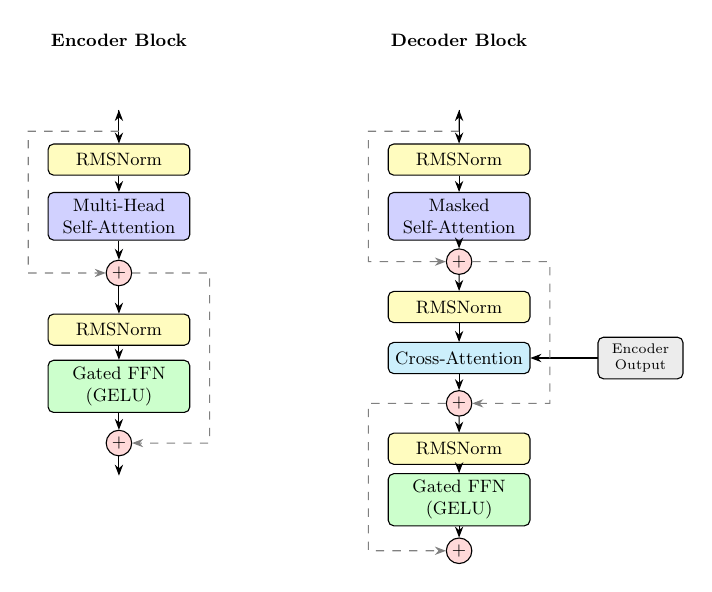
\begin{tikzpicture}[
    scale=0.72,
    transform shape,
    block/.style={draw, rectangle, minimum width=2.5cm, minimum height=0.55cm,
        align=center, rounded corners=2pt, font=\small},
    norm/.style={block, fill=yellow!25},
    attn/.style={block, fill=blue!18},
    ffn/.style={block, fill=green!20},
    add/.style={draw, circle, minimum size=0.45cm, fill=red!15, inner sep=0pt,
        font=\small\bfseries},
    arrow/.style={-{Stealth[length=4pt]}},
]

% ===== ENCODER BLOCK =====
\node[font=\small\bfseries] at (0, 8.3) {Encoder Block};

\node (enc_in) at (0, 7.2) {};
\draw[arrow] (0, 6.7) -- (enc_in);

\node[norm] (en1) at (0, 6.2) {RMSNorm};
\node[attn] (ea)  at (0, 5.2) {Multi-Head\\Self-Attention};
\node[add]  (ep1) at (0, 4.2) {$+$};
\node[norm] (en2) at (0, 3.2) {RMSNorm};
\node[ffn]  (ef)  at (0, 2.2) {Gated FFN\\(\gelu)};
\node[add]  (ep2) at (0, 1.2) {$+$};
\node (enc_out) at (0, 0.5) {};

\draw[arrow] (enc_in) -- (en1);
\draw[arrow] (en1) -- (ea);
\draw[arrow] (ea) -- (ep1);
\draw[arrow] (ep1) -- (en2);
\draw[arrow] (en2) -- (ef);
\draw[arrow] (ef) -- (ep2);
\draw[arrow] (ep2) -- (enc_out);

% Residual connections
\draw[arrow, gray, dashed] (0,6.7) -- (-1.6,6.7) -- (-1.6,4.2) -- (ep1.west);
\draw[arrow, gray, dashed] (ep1.east) -- (1.6,4.2) -- (1.6,1.2) -- (ep2.east);

% ===== DECODER BLOCK =====
\node[font=\small\bfseries] at (6, 8.3) {Decoder Block};

\node (dec_in) at (6, 7.2) {};
\draw[arrow] (6, 6.7) -- (dec_in);

\node[norm] (dn1) at (6, 6.2) {RMSNorm};
\node[attn] (da1) at (6, 5.2) {Masked\\Self-Attention};
\node[add]  (dp1) at (6, 4.4) {$+$};
\node[norm] (dn2) at (6, 3.6) {RMSNorm};
\node[attn, fill=cyan!20] (da2) at (6, 2.7) {Cross-Attention};
\node[add]  (dp2) at (6, 1.9) {$+$};
\node[norm] (dn3) at (6, 1.1) {RMSNorm};
\node[ffn]  (df)  at (6, 0.2) {Gated FFN\\(\gelu)};
\node[add]  (dp3) at (6, -0.7) {$+$};

\draw[arrow] (dec_in) -- (dn1);
\draw[arrow] (dn1) -- (da1);
\draw[arrow] (da1) -- (dp1);
\draw[arrow] (dp1) -- (dn2);
\draw[arrow] (dn2) -- (da2);
\draw[arrow] (da2) -- (dp2);
\draw[arrow] (dp2) -- (dn3);
\draw[arrow] (dn3) -- (df);
\draw[arrow] (df) -- (dp3);

% Encoder memory input
\node[block, fill=gray!15, minimum width=1.5cm, font=\scriptsize] (mem) at (9.2, 2.7) {Encoder\\Output};
\draw[arrow] (mem) -- (da2);

% Residual connections
\draw[arrow, gray, dashed] (6,6.7) -- (4.4,6.7) -- (4.4,4.4) -- (dp1.west);
\draw[arrow, gray, dashed] (dp1.east) -- (7.6,4.4) -- (7.6,1.9) -- (dp2.east);
\draw[arrow, gray, dashed] (dp2.west) -- (4.4,1.9) -- (4.4,-0.7) -- (dp3.west);

\end{tikzpicture}
\caption{Pre-LN Transformer blocks. \textbf{Left}: Encoder block with self-attention and gated FFN. \textbf{Right}: Decoder block adding masked self-attention and cross-attention to encoder memory. RMSNorm is applied \emph{before} each sublayer (Pre-LN). Dashed gray arrows show residual connections.}
\label{fig:blocks}
\end{figure}

The encoder block computes:
\begin{align}
    \bm{x}' &= \bm{x} + \text{SelfAttn}(\rmsnorm(\bm{x})) \label{eq:enc_attn} \\
    \bm{x}'' &= \bm{x}' + \text{FFN}(\rmsnorm(\bm{x}')) \label{eq:enc_ffn}
\end{align}

The decoder block adds cross-attention between the two sublayers:
\begin{align}
    \bm{y}' &= \bm{y} + \text{MaskedSelfAttn}(\rmsnorm(\bm{y})) \\
    \bm{y}'' &= \bm{y}' + \text{CrossAttn}(\rmsnorm(\bm{y}'), \bm{h}_\text{enc}) \\
    \bm{y}''' &= \bm{y}'' + \text{FFN}(\rmsnorm(\bm{y}''))
\end{align}

where $\bm{h}_\text{enc}$ is the encoder output.
Hidden states are clamped to prevent overflow during mixed-precision (bfloat16) training, following the HuggingFace T5 implementation.

\subsection{Multi-Head Attention}
\label{sec:attention}

Attention is the mechanism that allows the model to dynamically focus on different parts of the input when producing each output element.
Given an input $\bm{X} \in \R^{n \times d}$, we project it into queries, keys, and values:
\begin{equation}
    \bm{Q} = \bm{X}\bm{W}_Q, \quad \bm{K} = \bm{X}\bm{W}_K, \quad \bm{V} = \bm{X}\bm{W}_V
\end{equation}
where $\bm{W}_Q, \bm{W}_K, \bm{W}_V \in \R^{d \times d_k}$.
In multi-head attention, we split each projection into $h$ heads of dimension $d_k = d / h$, compute attention independently per head, and concatenate:
\begin{equation}
    \text{MultiHead}(\bm{X}) = \text{Concat}(\text{head}_1, \ldots, \text{head}_h)\,\bm{W}_O
\end{equation}

Each head computes:
\begin{equation}
\label{eq:attention}
    \text{head}_i = \softmax\!\left(\bm{Q}_i \bm{K}_i^\top + \bm{B}_\text{rel}\right) \bm{V}_i
\end{equation}

\textbf{Note on scaling.}
The original Transformer~\citep{vaswani2017attention} scales attention scores by $1/\sqrt{d_k}$ to prevent softmax saturation.
T5 omits this scaling factor---the attention scores in Eq.~\eqref{eq:attention} are \emph{not} divided by $\sqrt{d_k}$.
\lexiname{} follows T5's convention via a configurable \texttt{scale\_scores} parameter.

\textbf{FlashAttention.}
When available, PyTorch~2.0's \texttt{scaled\_dot\_product\_attention} is used, which automatically selects the optimal kernel---FlashAttention~v2~\citep{dao2022flashattention}, memory-efficient attention, or a math fallback---based on hardware capabilities.
This reduces memory from $O(n^2)$ to $O(n)$ in the fused case.

Figure~\ref{fig:attention} illustrates the attention computation flow.

\begin{figure}[t]
\centering
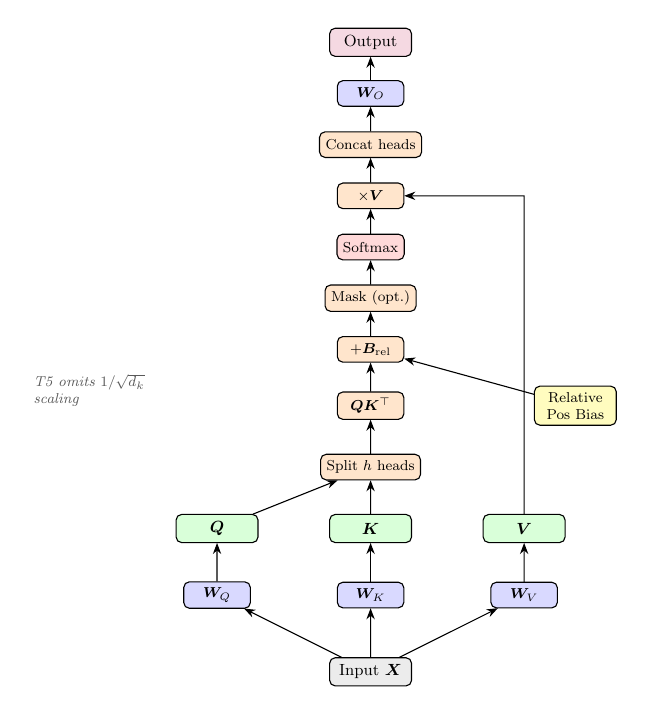
\begin{tikzpicture}[
    scale=0.65,
    transform shape,
    box/.style={draw, rectangle, minimum width=1.6cm, minimum height=0.55cm,
        align=center, rounded corners=2pt, font=\small},
    proj/.style={draw, rectangle, minimum width=1.3cm, minimum height=0.5cm,
        align=center, fill=blue!15, rounded corners=2pt, font=\footnotesize},
    op/.style={draw, rectangle, minimum width=1.3cm, minimum height=0.5cm,
        align=center, fill=orange!20, rounded corners=2pt, font=\footnotesize},
    arrow/.style={-{Stealth[length=4pt]}},
]

% Input
\node[box, fill=gray!15] (input) at (0, 0) {Input $\bm{X}$};

% Projections
\node[proj] (wq) at (-3, 1.5) {$\bm{W}_Q$};
\node[proj] (wk) at (0, 1.5) {$\bm{W}_K$};
\node[proj] (wv) at (3, 1.5) {$\bm{W}_V$};

% Q, K, V
\node[box, fill=green!15] (q) at (-3, 2.8) {$\bm{Q}$};
\node[box, fill=green!15] (k) at (0, 2.8) {$\bm{K}$};
\node[box, fill=green!15] (v) at (3, 2.8) {$\bm{V}$};

% Split heads
\node[op] (split) at (0, 4) {Split $h$ heads};

% Attention scores
\node[op] (matmul1) at (0, 5.2) {$\bm{Q}\bm{K}^\top$};

% Position bias
\node[box, fill=yellow!25, font=\footnotesize] (bias) at (4, 5.2) {Relative\\Pos Bias};

% Add bias
\node[op] (add) at (0, 6.3) {$+ \bm{B}_\text{rel}$};

% Mask
\node[op] (mask) at (0, 7.3) {Mask (opt.)};

% Softmax
\node[op, fill=red!15] (softmax) at (0, 8.3) {Softmax};

% MatMul with V
\node[op] (matmul2) at (0, 9.3) {$\times \bm{V}$};

% Concat
\node[op] (concat) at (0, 10.3) {Concat heads};

% Output projection
\node[proj] (wo) at (0, 11.3) {$\bm{W}_O$};

% Output
\node[box, fill=purple!15] (output) at (0, 12.3) {Output};

% Arrows
\draw[arrow] (input) -- (wq);
\draw[arrow] (input) -- (wk);
\draw[arrow] (input) -- (wv);
\draw[arrow] (wq) -- (q);
\draw[arrow] (wk) -- (k);
\draw[arrow] (wv) -- (v);
\draw[arrow] (q) -- (split);
\draw[arrow] (k) -- (split);
\draw[arrow] (v.north) -- ++(0,0.3) -| (3, 9.3) -- (matmul2);
\draw[arrow] (split) -- (matmul1);
\draw[arrow] (matmul1) -- (add);
\draw[arrow] (bias) -- (add);
\draw[arrow] (add) -- (mask);
\draw[arrow] (mask) -- (softmax);
\draw[arrow] (softmax) -- (matmul2);
\draw[arrow] (matmul2) -- (concat);
\draw[arrow] (concat) -- (wo);
\draw[arrow] (wo) -- (output);

% Annotation
\node[font=\footnotesize\itshape, align=left, text=gray!70!black] at (-5.5, 5.5) {T5 omits $1/\sqrt{d_k}$\\scaling};

\end{tikzpicture}
\caption{Multi-head attention with T5-style relative position bias. Attention scores are computed as $\bm{Q}\bm{K}^\top + \bm{B}_\text{rel}$, where $\bm{B}_\text{rel}$ is a learned bias indexed by the relative distance between query and key positions. T5 does \emph{not} scale by $1/\sqrt{d_k}$.}
\label{fig:attention}
\end{figure}

\subsubsection{Relative Position Bias}

Instead of absolute positional embeddings added to token representations, T5 encodes position information as a bias added directly to attention scores.
The relative position between positions $i$ and $j$ is mapped to a discrete bucket via logarithmic spacing:
\begin{equation}
    B_{ij} = \text{Embedding}\bigl[\text{bucket}(i - j)\bigr]
\end{equation}

Half the buckets encode exact positions for nearby tokens (distances 0--7), while the remaining half use logarithmic spacing for distant tokens (up to 128).
This allows the model to distinguish fine-grained local relationships while still representing long-range dependencies, all without adding parameters to the hidden states.

\textbf{An important detail}: in T5, only the first encoder layer and first decoder layer compute relative position biases.
These biases are then reused (broadcast) across all subsequent layers, rather than computing independent biases per layer.

\subsection{Gated Feed-Forward Network}

Following T5, \lexiname{} uses a \emph{gated} feed-forward network with GELU activation~\citep{hendrycks2016gelu}:
\begin{equation}
\label{eq:gated_ffn}
    \text{FFN}(\bm{x}) = \bigl(\gelu(\bm{x}\bm{W}_\text{gate}) \odot \bm{x}\bm{W}_\text{up}\bigr)\,\bm{W}_\text{down}
\end{equation}
where $\bm{W}_\text{gate}, \bm{W}_\text{up} \in \R^{d \times d_\text{ff}}$ and $\bm{W}_\text{down} \in \R^{d_\text{ff} \times d}$.
The gating mechanism ($\gelu \odot$) allows the network to selectively suppress information, providing more expressive transformations than the standard two-layer FFN.
With $d = 768$ and $d_\text{ff} = 2048$, each gated FFN has three weight matrices instead of two, giving $3 \times 768 \times 2048 \approx 4.7$M parameters per block.

\subsection{RMSNorm}

RMSNorm normalizes by the root mean square only, dropping the mean-centering operation of standard LayerNorm:
\begin{equation}
    \rmsnorm(\bm{x}) = \frac{\bm{x}}{\sqrt{\frac{1}{d}\sum_{i=1}^{d} x_i^2 + \epsilon}} \cdot \bm{\gamma}
\end{equation}

where $\bm{\gamma} \in \R^d$ is a learned scale parameter and $\epsilon = 10^{-6}$.
There is no bias term.
This is computationally cheaper than LayerNorm (one fewer reduction) and empirically performs comparably~\citep{zhang2019root}.

\subsection{Task-Specific Heads}
\label{sec:heads}

The shared encoder produces contextualized representations $\bm{H} \in \R^{n \times d}$.
Different tasks consume these representations through different heads.

\subsubsection{Summarization: Decoder + LM Head}

Summarization uses the full encoder--decoder pipeline.
Encoder outputs $\bm{H}$ are passed to the decoder via cross-attention, and the decoder autoregressively generates summary tokens.
The language modeling head projects decoder hidden states to vocabulary logits, \emph{with weights tied to the token embedding matrix}:
\begin{equation}
    P(y_t \mid y_{<t}, \bm{x}) = \softmax(\bm{h}_t^{\text{dec}} \bm{W}_\text{embed}^\top)
\end{equation}

Training uses cross-entropy loss with label smoothing ($\epsilon = 0.1$) and \texttt{ignore\_index=-100} for padding tokens.
Inference uses greedy decoding with a maximum length of 128 tokens.

\subsubsection{Emotion Classification: Attention Pooling + MLP}
\label{sec:emotion_head}

Emotion detection is a 28-label multi-label classification task---each text may express multiple emotions simultaneously.
A naive approach would mean-pool the encoder outputs, but emotional content is typically concentrated in specific tokens or phrases, and mean pooling dilutes these signals across the full sequence.

Instead, we use \emph{learned attention pooling}: a trainable weight vector $\bm{w} \in \R^d$ computes a per-position scalar score, and the output is a weighted sum of encoder hidden states:
\begin{align}
    \alpha_i &= \frac{\exp(\bm{w}^\top \bm{h}_i)}{\sum_{j \in \text{valid}} \exp(\bm{w}^\top \bm{h}_j)} \\
    \bm{h}_\text{pool} &= \sum_{i \in \text{valid}} \alpha_i \, \bm{h}_i
\end{align}
where ``valid'' denotes non-padding positions.
This allows the model to attend to emotionally salient tokens rather than treating all positions equally.

The pooled representation is then passed through a two-layer MLP:
\begin{equation}
    \text{logits} = \bm{W}_2\,\gelu(\bm{W}_1\,\bm{h}_\text{pool} + \bm{b}_1) + \bm{b}_2
\end{equation}
where $\bm{W}_1 \in \R^{d/2 \times d}$ and $\bm{W}_2 \in \R^{28 \times d/2}$, giving a hidden dimension of 384.
The MLP provides additional nonlinear capacity for the challenging 28-label task.

Training uses binary cross-entropy with logits loss (BCEWithLogitsLoss), enabling independent per-label prediction.
At inference, per-label sigmoid probabilities are thresholded at 0.5 (or per-class tuned thresholds) to produce multi-label predictions.

\subsubsection{Topic Classification: Mean Pooling + Linear}

Topic classification assigns each document to exactly one of 7 categories: Arts, Business, Fiction, History, Philosophy, Science, and Technology.
Because topical information is distributed more uniformly across the text (unlike emotion), simple mean pooling is effective:
\begin{equation}
    \bm{h}_\text{pool} = \frac{\sum_{i=1}^{n} m_i \, \bm{h}_i}{\sum_{i=1}^{n} m_i}
\end{equation}
where $m_i \in \{0, 1\}$ is the attention mask.
A single linear layer projects to 7-way logits, trained with standard cross-entropy loss.

% =====================================================================
\section{Weight Transfer from FLAN-T5}
\label{sec:weight_transfer}
% =====================================================================

A key design goal of \lexiname{} is to combine the transparency of a custom implementation with the linguistic knowledge of a pre-trained model.
The \texttt{factory.py} module handles this through a three-step pipeline: \textbf{(1)}~load configuration, \textbf{(2)}~instantiate custom modules, \textbf{(3)}~map and transfer pre-trained weights.

\subsection{Configuration}

Architecture hyperparameters are defined in a YAML configuration file and loaded into a \texttt{ModelConfig} dataclass.
Table~\ref{tab:model_specs} lists the values for the base configuration.

\begin{table}[t]
\centering
\caption{\lexiname{} model specifications (base configuration).}
\label{tab:model_specs}
\begin{tabular}{lc}
\toprule
\textbf{Parameter} & \textbf{Value} \\
\midrule
Hidden dimension ($d_\text{model}$) & 768 \\
FFN dimension ($d_\text{ff}$) & 2048 \\
Attention heads ($h$) & 12 \\
Head dimension ($d_k$) & 64 \\
Encoder layers ($N_\text{enc}$) & 12 \\
Decoder layers ($N_\text{dec}$) & 12 \\
Vocabulary size & 32{,}128 \\
Max sequence length & 512 \\
Dropout & 0.1 \\
Activation & Gated-GELU \\
Normalization & RMSNorm (Pre-LN) \\
Position encoding & Relative bias \\
\midrule
Total parameters & $\sim$272M \\
\bottomrule
\end{tabular}
\end{table}

\subsection{Weight Mapping}

The pre-trained \tflant{}-base model uses HuggingFace's naming convention, which differs from our custom parameter names.
The factory module maps between the two:

\begin{table}[t]
\centering
\caption{Weight mapping from \tflant{} to \lexiname{}. The mapping is defined explicitly in \texttt{factory.py}, enabling transparent verification that all parameters are transferred.}
\label{tab:weight_mapping}
\small
\begin{tabular}{@{}ll@{}}
\toprule
\textbf{\tflant{} Parameter} & \textbf{\lexiname{} Parameter} \\
\midrule
\texttt{shared} & \texttt{encoder.embedding} \\
\texttt{*.SelfAttention.q} & \texttt{*.self\_attn.W\_Q} \\
\texttt{*.SelfAttention.k} & \texttt{*.self\_attn.W\_K} \\
\texttt{*.SelfAttention.v} & \texttt{*.self\_attn.W\_V} \\
\texttt{*.SelfAttention.o} & \texttt{*.self\_attn.W\_O} \\
\texttt{*.layer\_norm} & \texttt{*.norm*} \\
\texttt{*.DenseReluDense.wi\_0} & \texttt{*.ffn.linear\_gate} \\
\texttt{*.DenseReluDense.wi\_1} & \texttt{*.ffn.linear1} \\
\texttt{*.DenseReluDense.wo} & \texttt{*.ffn.linear2} \\
\texttt{lm\_head} & \texttt{decoder.output\_projection} \\
\bottomrule
\end{tabular}
\end{table}

\subsection{Vocabulary Size Handling}

T5 pads its vocabulary to multiples of 128 for GPU efficiency: the ``real'' vocabulary is 32{,}100 tokens, but the embedding matrix has 32{,}128 rows.
During weight transfer, we copy only the tokens that exist in both vocabularies and initialize any extra rows with small random values.

\subsection{Bias Initialization}

T5's attention layers have no bias terms, but our implementation includes optional biases for generality.
When transferring weights, these bias terms are zero-initialized to ensure functional equivalence with the pre-trained model.

% =====================================================================
\section{Multi-Task Learning}
\label{sec:multitask}
% =====================================================================

The \texttt{MultiTaskModel} class routes inputs to the appropriate processing path based on head type.
Figure~\ref{fig:routing} illustrates the routing logic.

\begin{figure}[t]
\centering
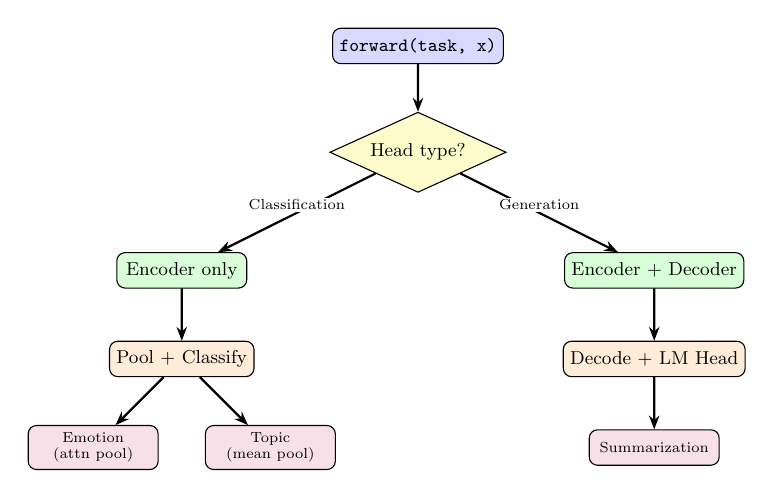
\begin{tikzpicture}[
    scale=0.75,
    transform shape,
    box/.style={draw, rectangle, minimum width=2.2cm, minimum height=0.6cm,
        align=center, rounded corners=3pt, font=\small},
    decision/.style={draw, diamond, aspect=2.2, minimum width=1.8cm,
        align=center, fill=yellow!20, font=\small},
    arrow/.style={-{Stealth[length=5pt]}, thick},
]

\node[box, fill=blue!15] (fwd) at (0, 0) {\texttt{forward(task, x)}};
\node[decision] (check) at (0, -1.8) {Head type?};

\node[box, fill=green!15] (enc) at (-4, -3.8) {Encoder only};
\node[box, fill=green!15] (s2s) at (4, -3.8) {Encoder + Decoder};

\node[box, fill=orange!15] (cls) at (-4, -5.3) {Pool + Classify};
\node[box, fill=orange!15] (lm) at (4, -5.3) {Decode + LM Head};

\node[box, fill=purple!12, font=\scriptsize] (e1) at (-5.5, -6.8) {Emotion\\(attn pool)};
\node[box, fill=purple!12, font=\scriptsize] (e2) at (-2.5, -6.8) {Topic\\(mean pool)};
\node[box, fill=purple!12, font=\scriptsize] (e3) at (4, -6.8) {Summarization};

\draw[arrow] (fwd) -- (check);
\draw[arrow] (check) -- (enc) node[midway, above, font=\scriptsize, fill=white, inner sep=1pt] {Classification};
\draw[arrow] (check) -- (s2s) node[midway, above, font=\scriptsize, fill=white, inner sep=1pt] {Generation};
\draw[arrow] (enc) -- (cls);
\draw[arrow] (s2s) -- (lm);
\draw[arrow] (cls) -- (e1);
\draw[arrow] (cls) -- (e2);
\draw[arrow] (lm) -- (e3);

\end{tikzpicture}
\caption{Task routing in \texttt{MultiTaskModel}. The head type determines whether encoder-only (classification) or full encoder--decoder (generation) processing is used.}
\label{fig:routing}
\end{figure}

\subsection{Temperature-Based Task Sampling}

When training on multiple tasks with different dataset sizes (49K summarization, 43K emotion, 3.4K topic), uniform sampling would cause the model to see far more summarization and emotion examples per epoch than topic examples.
We use temperature-based sampling~\citep{arivazhagan2019massively} to balance task exposure:
\begin{equation}
    p_t = \frac{|D_t|^{1/\alpha}}{\sum_{t'} |D_{t'}|^{1/\alpha}}
\end{equation}
where $|D_t|$ is the size of dataset $t$ and $\alpha$ is the temperature parameter.
With $\alpha = 0.5$ (our setting), smaller datasets are upsampled relative to their natural frequency, preventing them from being overwhelmed by larger tasks.

\subsection{Task Loss Weighting}

The total loss combines task-specific losses with explicit weights:
\begin{equation}
    \mathcal{L}_\text{total} = \lambda_\text{summ}\,\mathcal{L}_\text{summ} + \lambda_\text{emo}\,\mathcal{L}_\text{emo} + \lambda_\text{topic}\,\mathcal{L}_\text{topic}
\end{equation}

We set $\lambda_\text{summ} = \lambda_\text{emo} = 1.0$ and $\lambda_\text{topic} = 0.3$.
The reduced topic weight prevents the small topic dataset from dominating shared gradients---without this, topic classification converges to near-perfect training accuracy within 2--3 epochs while degrading performance on other tasks.

% =====================================================================
\section{Training Pipeline}
\label{sec:training}
% =====================================================================

\subsection{Datasets}
\label{sec:datasets}

Table~\ref{tab:datasets} summarizes the training data for each task.

\begin{table}[t]
\centering
\caption{Dataset statistics. All splits use consistent tokenization with a maximum length of 512 tokens.}
\label{tab:datasets}
\small
\begin{tabular}{@{}llrrr@{}}
\toprule
\textbf{Task} & \textbf{Source} & \textbf{Train} & \textbf{Val} & \textbf{Test} \\
\midrule
\multirow{3}{*}{Summarization} & Gutenberg + Goodreads & 4K & -- & -- \\
 & arXiv (body $\to$ abstract) & 45K & -- & -- \\
 & \textit{Combined} & 49,086 & 2,727 & 2,727 \\
\midrule
Topic (7-class) & 20News + Gut.\ + arXiv & 3,402 & 189 & 189 \\
\midrule
Emotion (28-label) & GoEmotions & 43,410 & 5,426 & 5,427 \\
\midrule
\multicolumn{2}{@{}l}{\textbf{Total}} & \textbf{95,898} & \textbf{8,342} & \textbf{8,343} \\
\bottomrule
\end{tabular}
\end{table}

\textbf{Summarization.}
Literary pairs match Project Gutenberg full texts with Goodreads back-cover descriptions via title/author matching.
Academic pairs use arXiv paper bodies with their abstracts.
The academic subset is substantially larger ($\sim$45K vs.\ $\sim$4K literary), creating an 11:1 domain imbalance that favors academic summarization quality (Section~\ref{sec:results}).

\textbf{Topic classification.}
Labels are derived from source metadata (arXiv categories, Gutenberg subjects, 20~Newsgroups categories) and mapped to a 7-class taxonomy.
No manual annotation was performed, introducing potential noise from metadata inaccuracies.

\textbf{Emotion detection.}
GoEmotions~\citep{demszky2020goemotions} provides 28 fine-grained emotion labels derived from Reddit comments.
The 28 labels are: admiration, amusement, anger, annoyance, approval, caring, confusion, curiosity, desire, disappointment, disapproval, disgust, embarrassment, excitement, fear, gratitude, grief, joy, love, nervousness, neutral, optimism, pride, realization, relief, remorse, sadness, and surprise.

\textbf{Cross-task deduplication.}
Because the topic dataset draws from the same sources as summarization (arXiv, Gutenberg), we perform cross-task document deduplication using MD5 fingerprints of normalized text prefixes to prevent data leakage.

\subsection{Tokenization}

\lexiname{} wraps HuggingFace's \texttt{AutoTokenizer} with a simplified fa\c{c}ade handling T5-specific conventions.
T5 uses SentencePiece~\citep{kudo2018sentencepiece} unigram tokenization with a 32{,}128-token vocabulary.
Notable conventions: \texttt{pad\_token\_id=0}, \texttt{eos\_token\_id=1}, no explicit BOS token (the pad token serves as the decoder start token).

For seq2seq training, decoder inputs are created by right-shifting the target labels:

\begin{lstlisting}[caption={Decoder input preparation},numbers=none]
decoder_inputs[:, 0] = bos_token_id  # = pad_token_id for T5
decoder_inputs[:, 1:] = labels[:, :-1]
\end{lstlisting}

\subsection{Training Configuration}

All training was conducted on a single NVIDIA RTX~4070 (12\,GB VRAM).
Table~\ref{tab:training_config} lists the hyperparameters.

\begin{table}[t]
\centering
\caption{Training hyperparameters.}
\label{tab:training_config}
\small
\begin{tabular}{@{}ll@{}}
\toprule
\textbf{Hyperparameter} & \textbf{Value} \\
\midrule
Optimizer & Fused AdamW \\
Learning rate & $3 \times 10^{-5}$ \\
Weight decay & 0.01 \\
Betas & (0.9, 0.98) \\
Batch size & 10 (effective 40 with 4$\times$ accum.) \\
LR schedule & Cosine with linear warmup \\
Warmup steps & 300 \\
Min LR ratio & 0.1$\times$ peak \\
Max epochs & 8 \\
Early stopping patience & 3 \\
Precision & BFloat16 (AMP) \\
Gradient clipping & Max norm 1.0 \\
Gradient checkpointing & Enabled \\
\texttt{torch.compile} & Encoder and decoder \\
Label smoothing & 0.1 (summarization) \\
Task weights & Summ.~1.0, Emo.~1.0, Topic~0.3 \\
Task sampling & Temperature ($\alpha = 0.5$) \\
Frozen encoder layers & Bottom 4 of 12 \\
\bottomrule
\end{tabular}
\end{table}

\textbf{Mixed-precision training.}
We use PyTorch AMP with BFloat16; on Ampere+ GPUs, bfloat16 provides better numerical stability than float16 (no loss scaling needed) while maintaining equivalent speed benefits.
TF32 is enabled for matrix multiplications.

\textbf{Learning rate schedule.}
A linear warmup over 300 steps ($\sim$0.5 epochs) prevents early training instability.
After warmup, the learning rate follows a cosine decay to 10\% of its peak value:
\begin{equation}
    \eta(t) = \eta_\text{min} + \tfrac{1}{2}(\eta_\text{max} - \eta_\text{min})\bigl(1 + \cos(\pi \cdot \text{progress})\bigr)
\end{equation}
where $\text{progress} = (t - t_\text{warmup}) / (T - t_\text{warmup})$ and $\eta_\text{min} = 0.1 \cdot \eta_\text{max}$.

\textbf{Encoder freezing.}
The bottom 4 encoder layers are frozen during fine-tuning.
These layers capture general linguistic features (morphology, syntax) that transfer well across tasks; freezing them preserves these representations while reducing memory and compute, and allowing upper layers to specialize for our domain.

\textbf{CUDA optimizations.}
We enable \texttt{cudnn.benchmark}, TF32 for matmul, FlashAttention via SDPA, and memory-efficient attention kernels.

% =====================================================================
\section{Experimental Results}
\label{sec:results}
% =====================================================================

We evaluate on held-out validation sets.
All summarization metrics report mean and 95\% bootstrap confidence intervals.
Training completed all 8 epochs (approximately 9~hours) without triggering early stopping.

\subsection{Summarization}

\begin{table}[t]
\centering
\caption{Summarization results on the validation set ($n = 2{,}727$).}
\label{tab:summ_results}
\begin{tabular}{lc}
\toprule
\textbf{Metric} & \textbf{Score} \\
\midrule
ROUGE-1 & 0.310~{\scriptsize[0.306, 0.313]} \\
ROUGE-2 & 0.091~{\scriptsize[0.088, 0.094]} \\
ROUGE-L & 0.185~{\scriptsize[0.182, 0.188]} \\
BLEU-4 & 0.024 \\
\midrule
BERTScore Precision & 0.843 \\
BERTScore Recall & 0.818 \\
\textbf{BERTScore F1} & \textbf{0.830} \\
\bottomrule
\end{tabular}
\end{table}

The high BERTScore F1 (0.83) combined with moderate ROUGE-1 (0.31) is characteristic of abstractive summarization: the model generates semantically faithful paraphrases rather than extracting text verbatim.
ROUGE, which measures n-gram overlap, undervalues such paraphrasing; BERTScore's contextual embeddings~\citep{zhang2019bertscore} better capture semantic similarity.

\textbf{Per-domain analysis.}
The 11:1 training imbalance produces a clear quality gap: academic summaries achieve ROUGE-1 of 0.319 while literary summaries reach only 0.206.
This is expected---the model sees far more academic text during training and the formal structure of academic abstracts provides clearer extractive cues.

\begin{table}[t]
\centering
\caption{Per-domain summarization performance.}
\label{tab:domain_breakdown}
\begin{tabular}{@{}lcrrc@{}}
\toprule
\textbf{Domain} & \textbf{N} & \textbf{ROUGE-1} & \textbf{ROUGE-L} & \textbf{BLEU-4} \\
\midrule
Academic & 2{,}493 & 0.319 & 0.189 & 0.026 \\
Literary & 234 & 0.206 & 0.137 & 0.008 \\
\bottomrule
\end{tabular}
\end{table}

\subsection{Topic Classification}

\begin{table}[t]
\centering
\caption{Topic classification results on the validation set ($n = 189$).}
\label{tab:topic_results}
\begin{tabular}{lc}
\toprule
\textbf{Metric} & \textbf{Score} \\
\midrule
\textbf{Accuracy} & \textbf{85.7\%}~{\scriptsize[80.4\%, 91.0\%]} \\
Macro F1 & 0.854 \\
\bottomrule
\end{tabular}
\end{table}

Table~\ref{tab:topic_breakdown} shows per-class performance.
Fiction and Business achieve near-perfect F1 ($\geq 0.97$), while Science shows the most confusion (F1 = 0.67)---error analysis reveals frequent misclassification as Technology, which is semantically plausible given that scientific papers often describe technical methods.

\begin{table}[t]
\centering
\caption{Per-class topic classification performance.}
\label{tab:topic_breakdown}
\begin{tabular}{lccc}
\toprule
\textbf{Topic} & \textbf{Precision} & \textbf{Recall} & \textbf{F1} \\
\midrule
Arts & 0.93 & 0.79 & 0.86 \\
Business & 0.97 & 1.00 & 0.98 \\
Fiction & 0.95 & 1.00 & 0.97 \\
History & 0.85 & 0.76 & 0.80 \\
Philosophy & 0.79 & 0.82 & 0.81 \\
Science & 0.57 & 0.80 & 0.67 \\
Technology & 0.89 & 0.89 & 0.89 \\
\midrule
\textit{Macro Avg} & 0.85 & 0.87 & 0.85 \\
\bottomrule
\end{tabular}
\end{table}

\subsection{Emotion Detection}

Emotion detection is evaluated with three complementary F1 metrics, as each captures different aspects of multi-label performance:

\begin{table}[t]
\centering
\caption{Emotion detection results on the validation set ($n = 5{,}426$). Default uses a fixed threshold of 0.3; tuned uses per-class thresholds optimized on the validation set.}
\label{tab:emotion_results}
\begin{tabular}{lcc}
\toprule
\textbf{Metric} & \textbf{Default ($\tau=0.3$)} & \textbf{Tuned} \\
\midrule
Sample-avg F1 & 0.352~{\scriptsize[0.340, 0.366]} & \textbf{0.503} \\
Macro F1 & 0.143 & \textbf{0.294} \\
Micro F1 & 0.443 & \textbf{0.486} \\
\bottomrule
\end{tabular}
\end{table}

At the default threshold, 15 of 28 emotion classes have zero F1.
These tend to be rare classes ($< 100$ support) or semantically subtle emotions (anger, annoyance, approval) that overlap with other labels.
Per-class threshold tuning---sweeping $\tau \in \{0.10, 0.15, \ldots, 0.85\}$ per class (16 candidates, step 0.05)---recovers non-zero performance for most classes, doubling macro F1 from 0.143 to 0.294.

\textbf{Important caveat}: thresholds are tuned on the same validation set used for model selection (early stopping), so tuned metrics are optimistically biased.
With 16 candidates per class, the effective search space is large enough to overfit to validation set idiosyncrasies, particularly for rare emotion classes.
The untuned results ($\tau = 0.3$) are not subject to this bias.
For rigorous evaluation, thresholds should be tuned on a held-out calibration split separate from both the validation set and the test set; we estimate the bias at 2--5\% based on the search space size.

The strongest classes are gratitude (F1 = 0.89), amusement (0.75), love (0.74), and admiration (0.65)---these have clear lexical signals and reasonable support ($> 250$ samples).
The model struggles most with rare, nuanced emotions like grief (13 samples), embarrassment (35), and pride (15).

\subsection{Training Dynamics}

Training completed 8 full epochs (no early stopping triggered).
Combined validation loss decreased monotonically from 4.297 (epoch~1) to 3.925 (epoch~8).
Validation emotion sample F1 rose steadily from 0.197 to 0.459, while topic accuracy plateaued after epoch~5 at $\sim$86\%.

The different learning trajectories illustrate a key MTL phenomenon: the small topic dataset saturates quickly (97\% training accuracy by epoch~3), while emotion detection---with its larger dataset and harder 28-class problem---continues improving throughout.
The reduced topic weight ($\lambda = 0.3$) and temperature sampling prevent the saturated topic task from degrading the shared encoder.

\subsection{Baseline Comparison: BERT}

To disentangle the effects of architecture from multi-task learning, we compare \lexiname{} against BERT-base-uncased~\citep{devlin2019bert} (110M parameters) in three configurations: single-task topic, single-task emotion, and joint multitask.
The BERT baselines use identical training hyperparameters (learning rate, batch size, gradient accumulation, epochs) and the same data splits, with task-specific classification heads matching \lexiname{}'s design: attention pooling + 2-layer MLP for emotion, mean pooling + linear projection for topic.

\begin{table}[t]
\centering
\caption{Comparison of \lexiname{} (encoder--decoder MTL) with BERT-base baselines.
Single-task models are trained on one task only; multitask trains on both classification tasks jointly.
Bold indicates best per metric; $\dagger$ denotes tuned per-class thresholds.}
\label{tab:bert_comparison}
\setlength{\tabcolsep}{3pt}
\small
\begin{tabular}{@{}lcccc@{}}
\toprule
& \lexiname{} & \textbf{BERT} & \textbf{BERT} & \textbf{BERT} \\
\textbf{Metric} & \textbf{(MTL)} & \textbf{Single} & \textbf{Single} & \textbf{MTL} \\
& & \textbf{Topic} & \textbf{Emotion} & \\
\midrule
\multicolumn{5}{@{}l}{\textit{Topic Classification}} \\
\quad Accuracy & 85.7\% & \textbf{87.3\%} & --- & 79.9\% \\
\quad Macro F1 & 0.854 & \textbf{0.878} & --- & 0.776 \\
\midrule
\multicolumn{5}{@{}l}{\textit{Emotion Detection}} \\
\quad Sample-avg F1 & 0.352 & --- & \textbf{0.608} & 0.607 \\
\quad Macro F1 & 0.143 & --- & \textbf{0.469} & 0.487 \\
\quad Micro F1 & 0.443 & --- & \textbf{0.607} & 0.600 \\
\quad Macro F1$^\dagger$ & 0.294 & --- & \textbf{0.512} & 0.510 \\
\midrule
\multicolumn{5}{@{}l}{\textit{Summarization}} \\
\quad BERTScore F1 & \textbf{0.830} & --- & --- & --- \\
\bottomrule
\end{tabular}
\end{table}

Table~\ref{tab:bert_comparison} reveals several instructive patterns:

\paragraph{BERT dominates classification.}
The encoder-only architecture substantially outperforms \lexiname{} on both classification tasks in single-task settings (+1.6\% topic accuracy, +72\% relative emotion sample F1).
This is expected: BERT's bidirectional encoder produces richer contextual representations for classification than using only the encoder half of an encoder--decoder model, and BERT can devote all parameters to the classification objective.

\paragraph{MTL hurts BERT on topic.}
BERT's multitask configuration drops topic accuracy by 7.4 percentage points compared to its single-task result (79.9\% vs.\ 87.3\%), while emotion performance remains essentially unchanged.
This mirrors the negative transfer \lexiname{} avoids through temperature sampling and attention pooling---the same interventions are absent in the BERT multitask setup.

\paragraph{Architecture enables generation.}
The BERT baselines cannot perform abstractive summarization---this capability requires the decoder component unique to \lexiname{}'s encoder--decoder design.
The classification performance gap is the cost of architectural flexibility: \lexiname{} uses a single model for all three tasks, including a generative task that encoder-only models cannot address.

% =====================================================================
\section{Discussion}
\label{sec:discussion}
% =====================================================================

\subsection{Why Attention Pooling Matters}

The choice of pooling mechanism for classification heads has outsized impact.
Mean pooling works well for topic classification because topical signals are distributed across the text---a paper about machine learning will contain relevant vocabulary throughout.
But emotional content is localized: a single phrase (``I'm devastated'') may carry all the emotional signal, diluted by hundreds of neutral tokens under mean pooling.

Learned attention pooling lets the model focus on these salient positions.
Switching from mean pooling to attention pooling for the emotion head---with no other changes---improved sample-averaged F1 from 0.199 to 0.352 (+77\%), completely eliminating the negative transfer observed in the naive MTL configuration.

\subsection{The BERTScore vs.\ ROUGE Gap}

The large gap between BERTScore F1 (0.83) and ROUGE-1 (0.31) deserves explanation.
ROUGE measures \emph{lexical} overlap---it counts shared n-grams between generated and reference texts.
BERTScore computes cosine similarity between contextual embeddings, capturing \emph{semantic} similarity regardless of exact wording.

For abstractive summarization, this gap is expected and even desirable: it means the model is paraphrasing (generating semantically equivalent text with different words) rather than copying.
Our summarization head generates back-cover style descriptions rather than extractive summaries, so high BERTScore with moderate ROUGE indicates the model is behaving as intended.

\subsection{Domain Imbalance in Summarization}

The 11:1 academic-to-literary training ratio produces a clear quality asymmetry: academic ROUGE-1 of 0.319 vs.\ literary ROUGE-1 of 0.206.
Beyond raw volume, academic text provides stronger extractive cues---paper abstracts follow predictable structures (``We propose\ldots'', ``Experiments show\ldots'') that transfer well to compression.
Literary descriptions are more open-ended, and the model's exposure to contemporary fiction is limited by Project Gutenberg's focus on pre-1928 public domain works.

\subsection{Limitations}

\begin{itemize}[nosep]
    \item \textbf{Classification--generation tradeoff}: The BERT baseline comparison (Table~\ref{tab:bert_comparison}) confirms that the encoder--decoder architecture underperforms encoder-only models on pure classification. This is the cost of supporting generative tasks within a single model.
    \item \textbf{Emotion--domain mismatch}: GoEmotions is sourced from Reddit comments, which differ sharply in register from the literary and academic content \lexiname{} targets. The 28-class multi-label setting compounds this difficulty.
    \item \textbf{Topic data scarcity}: With only 3{,}402 training samples across 7 classes, some categories (notably Science, F1~=~0.67) lack sufficient examples. The Science--Technology boundary is inherently ambiguous.
    \item \textbf{Literary generation quality}: The domain imbalance limits literary summarization. Balancing the training mix or augmenting with contemporary book data would likely help.
    \item \textbf{Greedy decoding}: We use greedy decoding for simplicity; beam search or nucleus sampling could improve generation diversity and quality.
\end{itemize}

\subsection{Future Directions}

\begin{itemize}[nosep]
    \item \textbf{LoRA}~\citep{hu2022lora}: Parameter-efficient fine-tuning would reduce memory requirements, enabling experimentation with FLAN-T5-large (780M) or FLAN-T5-xl (3B).
    \item \textbf{Domain-specific emotion data}: Training on literary emotion annotations rather than Reddit comments would better capture the emotional register of books and papers.
    \item \textbf{Threshold learning}: Replacing the fixed sigmoid threshold with a learned decision boundary per class could improve multi-label performance without post-hoc tuning.
    \item \textbf{Data augmentation}: Back-translation or LLM-based paraphrasing for the small topic dataset could improve classification robustness.
\end{itemize}

% =====================================================================
\section{Conclusion}
\label{sec:conclusion}
% =====================================================================

We presented \lexiname{}, a multi-task NLP system that combines a custom Transformer reimplementation with \tflant{} pre-trained weights.
The hybrid approach provides full architectural transparency while leveraging transfer learning, achieving:

\begin{itemize}[nosep]
    \item \textbf{Summarization}: BERTScore F1 of 0.83, demonstrating strong semantic fidelity for abstractive literary and academic summaries.
    \item \textbf{Topic Classification}: 85.7\% accuracy (macro F1 = 0.854) across 7 categories.
    \item \textbf{Emotion Detection}: Sample-averaged F1 of 0.352 (tuned macro F1 = 0.294) on 28 emotion labels.
\end{itemize}

Two interventions proved critical for balanced multi-task learning: learned attention pooling for the emotion head, and temperature-based task sampling.
Together, these eliminated negative transfer and improved emotion F1 by 77\% over the naive MTL baseline.

A controlled BERT-base comparison (Table~\ref{tab:bert_comparison}) clarifies the architecture tradeoff: BERT achieves stronger classification performance (87.3\% topic accuracy, 0.608 emotion sample F1) but cannot perform abstractive summarization.
The encoder--decoder design sacrifices classification accuracy in exchange for generative capabilities---a deliberate tradeoff that makes \lexiname{} suitable for applications requiring both understanding and generation.

The complete system trains in approximately 9~hours on a consumer GPU (NVIDIA RTX~4070, 12\,GB), demonstrating that sophisticated multi-task models remain accessible without datacenter-scale resources.
All code, trained weights, and datasets are publicly available.

% =====================================================================
% References
% =====================================================================

\bibliographystyle{plainnat}

\begin{thebibliography}{99}

\bibitem[Devlin et~al.(2019)]{devlin2019bert}
J.~Devlin, M.-W.~Chang, K.~Lee, and K.~Toutanova.
\newblock {BERT}: Pre-training of deep bidirectional transformers for language understanding.
\newblock In \emph{Proceedings of NAACL-HLT}, pages 4171--4186, 2019.

\bibitem[Vaswani et~al.(2017)]{vaswani2017attention}
A.~Vaswani, N.~Shazeer, N.~Parmar, J.~Uszkoreit, L.~Jones, A.~N.~Gomez, {\L}.~Kaiser, and I.~Polosukhin.
\newblock Attention is all you need.
\newblock In \emph{Advances in Neural Information Processing Systems (NeurIPS)}, volume~30, pages 5998--6008, 2017.

\bibitem[Raffel et~al.(2020)]{raffel2020exploring}
C.~Raffel, N.~Shazeer, A.~Roberts, K.~Lee, S.~Narang, M.~Matena, Y.~Zhou, W.~Li, and P.~J.~Liu.
\newblock Exploring the limits of transfer learning with a unified text-to-text transformer.
\newblock \emph{Journal of Machine Learning Research}, 21(140):1--67, 2020.

\bibitem[Chung et~al.(2022)]{chung2022scaling}
H.~W.~Chung, L.~Hou, S.~Longpre, B.~Zoph, Y.~Tay, W.~Fedus, et~al.
\newblock Scaling instruction-finetuned language models.
\newblock \emph{arXiv preprint arXiv:2210.11416}, 2022.

\bibitem[Xiong et~al.(2020)]{xiong2020layer}
R.~Xiong, Y.~Yang, J.~He, K.~Zheng, S.~Zheng, C.~Xing, H.~Zhang, Y.~Lan, L.~Wang, and T.~Liu.
\newblock On layer normalization in the transformer architecture.
\newblock In \emph{International Conference on Machine Learning (ICML)}, pages 10524--10533, 2020.

\bibitem[Zhang and Sennrich(2019)]{zhang2019root}
B.~Zhang and R.~Sennrich.
\newblock Root mean square layer normalization.
\newblock In \emph{Advances in Neural Information Processing Systems (NeurIPS)}, volume~32, pages 12360--12371, 2019.

\bibitem[Ba et~al.(2016)]{ba2016layer}
J.~L.~Ba, J.~R.~Kiros, and G.~E.~Hinton.
\newblock Layer normalization.
\newblock \emph{arXiv preprint arXiv:1607.06450}, 2016.

\bibitem[Caruana(1997)]{caruana1997multitask}
R.~Caruana.
\newblock Multitask learning.
\newblock \emph{Machine Learning}, 28(1):41--75, 1997.

\bibitem[Kudo and Richardson(2018)]{kudo2018sentencepiece}
T.~Kudo and J.~Richardson.
\newblock {SentencePiece}: A simple and language independent subword tokenizer and detokenizer for neural text processing.
\newblock In \emph{Proceedings of EMNLP: System Demonstrations}, pages 66--71, 2018.

\bibitem[Hu et~al.(2022)]{hu2022lora}
E.~J.~Hu, Y.~Shen, P.~Wallis, Z.~Allen-Zhu, Y.~Li, S.~Wang, L.~Wang, and W.~Chen.
\newblock {LoRA}: Low-rank adaptation of large language models.
\newblock In \emph{International Conference on Learning Representations (ICLR)}, 2022.

\bibitem[Dao et~al.(2022)]{dao2022flashattention}
T.~Dao, D.~Fu, S.~Ermon, A.~Rudra, and C.~R\'e.
\newblock {FlashAttention}: Fast and memory-efficient exact attention with {IO}-awareness.
\newblock In \emph{Advances in Neural Information Processing Systems (NeurIPS)}, volume~35, pages 16344--16359, 2022.

\bibitem[Demszky et~al.(2020)]{demszky2020goemotions}
D.~Demszky, D.~Movshovitz-Attias, J.~Ko, A.~Cowen, G.~Nemade, and S.~Ravi.
\newblock {GoEmotions}: A dataset of fine-grained emotions.
\newblock In \emph{Proceedings of ACL}, pages 4040--4054, 2020.

\bibitem[Zhang et~al.(2020)]{zhang2019bertscore}
T.~Zhang, V.~Kishore, F.~Wu, K.~Q.~Weinberger, and Y.~Artzi.
\newblock {BERTScore}: Evaluating text generation with {BERT}.
\newblock In \emph{International Conference on Learning Representations (ICLR)}, 2020.

\bibitem[Hendrycks and Gimpel(2016)]{hendrycks2016gelu}
D.~Hendrycks and K.~Gimpel.
\newblock {Gaussian Error Linear Units (GELUs)}.
\newblock \emph{arXiv preprint arXiv:1606.08415}, 2016.

\bibitem[Arivazhagan et~al.(2019)]{arivazhagan2019massively}
N.~Arivazhagan, A.~Bapna, O.~Firat, D.~Lepikhin, M.~Johnson, M.~Krikun, et~al.
\newblock Massively multilingual neural machine translation in the wild: Findings and challenges.
\newblock \emph{arXiv preprint arXiv:1907.05019}, 2019.

\end{thebibliography}

\end{document}
